$\zeta=\sympy{zeta}$, $\nu=\sympy{nu}$.

Найдём распределение случайной величины $\zeta$:

\begin{sympycode}
zeta1=zeta.subs(xi, x)
supp_zeta = ImageSet(Lambda(x, zeta1), x_interval)
supp_zeta1 = supp_zeta.simplify()
\end{sympycode}

Носитель случайной величины $\zeta$:
\[
    \supp \zeta = \sympy{supp_zeta} = \sympy{supp_zeta1}
\]

\begin{figure}[h!]
    \centering
    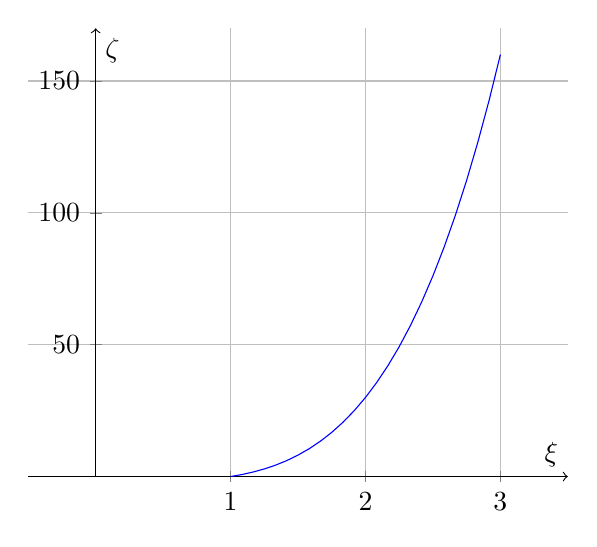
\begin{tikzpicture}
        \begin{axis}[
                xlabel=$\xi$,
                ylabel=$\zeta$,
                xmin=-0.5, xmax=3.5,
                ymin=0, ymax=170,
                axis lines=middle,
                axis line style={->},
                % ticks=none,
                % clip=true,
                % xtick={-1,-0.5,0,0.5,1},
                % ytick={-3,-2,-1,0,1,2,3},
                grid=both,
            ]
            \addplot[domain=1:3, blue, solid] {2 * x^4 - 2};
        \end{axis}
    \end{tikzpicture}
    \caption{График величины $\zeta$ в зависимости от $\xi$}
    \label{fig:zeta}
\end{figure}
\begin{sympycode}
x_by_z = solve(z - zeta1, x)[-1]
\end{sympycode}
1) $\zeta \in \sympy{supp_zeta1} \Rightarrow \xi \in \sympy{x_interval}$
\[
    A = \sympy{x_interval} \Rightarrow
    \begin{cases}
        g(x) = \sympy{zeta1}, \\
        g^{-1}(z) = \sympy{x_by_z}.
    \end{cases}
\]
\begin{sympycode}
x_by_z_derive = diff(x_by_z, z)
p_xi_sub_xz = p_xi.subs(x, x_by_z)
p_zeta = (x_by_z_derive * p_xi_sub_xz).simplify()
\end{sympycode}
\[
    p_\zeta
    = |(g^{-1}(z))'| \cdot p_{\xi} (g^{-1}(z))
    = \sympy{x_by_z_derive} \cdot \left(\sympy{p_xi_sub_xz}\right)
    = \sympy{p_zeta},
    z \in \sympy{supp_zeta1}.
\]

Итого, плотность распределения случайной величины $\zeta$:

\[
    p_\zeta (z)
    = \begin{cases}
        \sympy{p_zeta}, & z \in \sympy{supp_zeta1}, \\
        0,              & \text{иначе}.
    \end{cases}
\]
Мат. ожидание и дисперсия случайной величины $\zeta$:
\begin{sympycode}
Expect_zeta = integrate(z * p_zeta, (z, supp_zeta1.start, supp_zeta1.end))
Expect_zeta1 = Expect_zeta.simplify()
Expect_zeta_square = integrate((z) ** 2 * p_zeta, (z, supp_zeta1.start, supp_zeta1.end))
Variance_zeta1 = Expect_zeta_square - Expect_zeta ** 2
\end{sympycode}
\[
    \begin{aligned}
        \Expect\zeta
         & = \int\limits_{\sympy{supp_zeta1.start}}^{\sympy{supp_zeta1.end}} z \cdot p_\zeta (z) \, dz
        = \int\limits_{\sympy{supp_zeta1.start}}^{\sympy{supp_zeta1.end}} z \cdot \sympy{p_zeta} \, dz
        = \sympy{Expect_zeta1},                                                                        \\
        \Variance\zeta
         & = \Expect\zeta^2 - \left(\Expect\zeta\right)^2
        = \int\limits_{\sympy{supp_zeta1.start}}^{\sympy{supp_zeta1.end}} z^2 \cdot p_\zeta (z) \, dz - \left(\Expect\zeta\right)^2
        = \sympy{Expect_zeta_square} - \left(\sympy{Expect_zeta}\right)^2
        = \sympy{Variance_zeta1}.
    \end{aligned}
\]

По плотности вычислим функцию распределения \(\zeta\):

\begin{sympycode}
p_zeta_piece = Piecewise((p_zeta, supp_zeta1.as_relational(z)), (0, True))
F_zeta2 = integrate(p_zeta, (z, supp_zeta1.start, z)).simplify()
F_zeta1 = Piecewise((0, z <= supp_zeta1.start),
                    (F_zeta2, And(supp_zeta1.start < z, z <= supp_zeta1.end)), 
                    (1, True))
F_zeta1 = piecewise_exclusive(F_zeta1)
\end{sympycode}

\[
    F_\zeta (z) =
    \int\limits_{\sympy{supp_zeta1.start}}^{z} p_\zeta (z) \, dz =
    \int\limits_{\sympy{supp_zeta1.start}}^{z} \sympy{p_zeta} \, dz =
    \sympy{F_zeta2}
    z \in \sympy{supp_zeta1}.
\]

\[F_\zeta(z) = \sympy{F_zeta1}\]

\begin{figure}[h!]
    \centering
    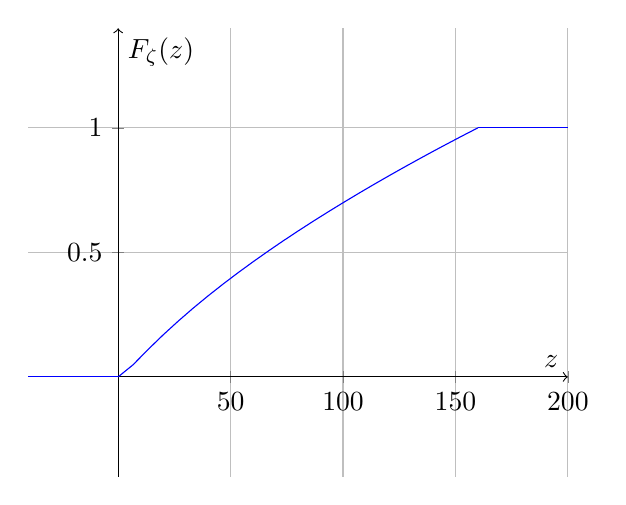
\begin{tikzpicture}
        \begin{axis}[
                xlabel=$z$,
                ylabel=$F_\zeta(z)$,
                % xmin=-0.5, xmax=170,
                ymin=-0.4, ymax=1.4,
                axis lines=middle,
                axis line style={->},
                % ticks=none,
                % clip=true,
                % xtick={-1,-0.5,0,0.5,1},
                % ytick={-3,-2,-1,0,1,2,3},
                grid=both,
            ]
            \addplot[domain=-40:0, blue, solid] {0};
            \addplot[domain=0:160, blue, solid]
            {(2^(1/2) * x + 2 * (x+2)^(1/2)*(-2^(3/4) * (x+2)^(1/4) + 1 ) + 2 * (2)^(1/2))/(8* (x+ 2)^(1/2))};
            \addplot[domain=160:200, blue, solid] {1};
        \end{axis}
    \end{tikzpicture}
    \caption{График функции распределения $F_\zeta(z)$}
    \label{fig:F_zeta}
\end{figure}
